
\section{Use Case}
\subsection{ UC1: Crea presentazione}

\begin{figure}[h]
	\begin{center}
	\includegraphics[scale=0.4]{diagram/UC1.png}
	\caption{Caso d'uso UC1}
	\end{center}
\end{figure}
\begin{itemize}
	\item \textbf{Precondizione:} l'utente ha effettuato l'accesso al sistema;
	\item \textbf{Postcondizione:} il sistema ha creato e salvato una nuova presentazione;
	\item \textbf{Descrizione:} l'utente potrà creare e salvare una presentazione che si aggiungerà alla lista delle presentazioni già create dallo stesso utente;
	\item \textbf{Attori:} Utente autenticato;
	\item \textbf{Scenario principale:}
	\begin{enumerate}
		\item \textbf{ UC1.1:} \textit{ Inserimento titolo};
		\item \textbf{ UC1.2:} \textit{ Inserimento descrizione}.
	\end{enumerate}
\end{itemize}
\subsection{ UC1.1: Inserimento titolo}

\begin{itemize}
	\item \textbf{Precondizione:} il sistema è in attesa che l'utente inserisca un titolo per la nuova presentazione;
	\item \textbf{Postcondizione:} il sistema ha inserito un titolo per la nuova presentazione;
	\item \textbf{Descrizione:} l'utente dopo aver scelto di creare una presentazione ne dovrà definire il titolo;
	\item \textbf{Attori:} Utente autenticato.
\end{itemize}
\subsection{ UC1.2: Inserimento descrizione}

\begin{itemize}
	\item \textbf{Precondizione:} il sistema è in attesa che l'utente inserisca una descrizione per la nuova presentazione;
	\item \textbf{Postcondizione:} il sistema ha inserito una descrizione per la nuova presentazione;
	\item \textbf{Descrizione:} l'utente dopo aver scelto di creare una presentazione potrà definirne una descrizione;
	\item \textbf{Attori:} Utente autenticato.
\end{itemize}
\subsection{ UC2: Selezione presentazione}

\begin{itemize}
	\item \textbf{Precondizione:} nel sistema deve essere presente almeno una presentazione creata dall'utente;
	\item \textbf{Postcondizione:} il sistema ha selezionato la presentazione scelta dall'utente;
	\item \textbf{Descrizione:} l'utente può selezionare una presentazione dall'elenco di quelle che ha creato;
	\item \textbf{Attori:} Utente autenticato.
\end{itemize}
\subsection{ UC3: Esegui presentazione}

\begin{figure}[h]
	\begin{center}
	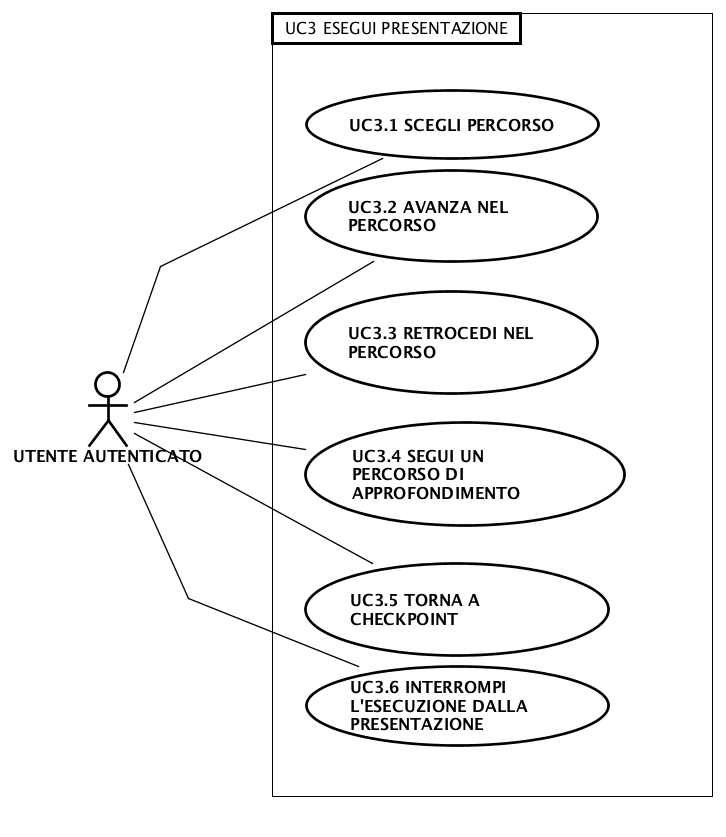
\includegraphics[scale=0.4]{diagram/UC3.png}
	\caption{Caso d'uso UC3}
	\end{center}
\end{figure}
\begin{itemize}
	\item \textbf{Precondizione:} il sistema ha selezionato la presentazione scelta dall'utente ed è in attesa di un’operazione da parte sua;
	\item \textbf{Postcondizione:} il sistema ha eseguito la presentazione scelta dall'utente;
	\item \textbf{Descrizione:} dopo aver selezionato una presentazione dall'elenco di quelle create l'utente potrà eseguirla;
	\item \textbf{Attori:} Utente autenticato;
	\item \textbf{Scenario principale:}
	\begin{enumerate}
		\item \textbf{ UC3.1:} \textit{ Scegli percorso};
		\item \textbf{ UC3.2:} \textit{ Avanza nel percorso};
		\item \textbf{ UC3.3:} \textit{ Retrocedi nel percorso};
		\item \textbf{ UC3.4:} \textit{ Segui un percorso di approfondimento};
		\item \textbf{ UC3.5:} \textit{ Torna a checkpoint};
		\item \textbf{ UC3.6:} \textit{ Interrompi esecuzione presentazione}.
	\end{enumerate}
\end{itemize}
\subsection{ UC3.1: Scegli percorso}

\begin{itemize}
	\item \textbf{Precondizione:} il sistema ha avviato la presentazione scelta dall'utente;
	\item \textbf{Postcondizione:} il sistema ha selezionato il percorso scelto dall'utente per la presentazione;
	\item \textbf{Descrizione:} l'utente può scegliere il percorso da effettuare in fase esecuzione della presentazione;
	\item \textbf{Attori:} Utente autenticato.
\end{itemize}
\subsection{ UC3.2: Avanza nel percorso}

\begin{itemize}
	\item \textbf{Precondizione:} il sistema è in fase di esecuzione della presentazione ed è in attesa di un'operazione da parte dell'utente;
	\item \textbf{Postcondizione:} il sistema ha fatto avanzare la presentazione di un passo ed il frame viene visualizzato;
	\item \textbf{Descrizione:} l'utente durante l'esecuzione della presentazione può avanzare la stessa di un passo, e viene aggiornata la visualizzazione del frame corrente;
	\item \textbf{Attori:} Utente autenticato.
\end{itemize}
\subsection{ UC3.3: Retrocedi nel percorso}

\begin{itemize}
	\item \textbf{Precondizione:} il sistema è in fase di esecuzione della presentazione ed è in attesa di un'operazione da parte dell'utente;
	\item \textbf{Postcondizione:} il sistema ha fatto retrocedere la presentazione di un passo ed il frame viene visualizzato;
	\item \textbf{Descrizione:} l'utente durante l'esecuzione della presentazione può far retrocedere la stessa di un passo, e viene aggiornata la visualizzazione del frame corrente;
	\item \textbf{Attori:} Utente autenticato.
\end{itemize}
\subsection{ UC3.4: Segui un percorso di approfondimento}

\begin{itemize}
	\item \textbf{Precondizione:} il sistema è in fase di esecuzione della presentazione ed è in attesa di un'operazione da parte dell'utente. Il frame attuale deve essere un checkpoint;
	\item \textbf{Postcondizione:} il sistema ha avanzato la presentazione in un percorso di approfondimento ed il frame viene visualizzato;
	\item \textbf{Descrizione:} l'utente può scegliere di intraprendere un percorso di approfondimento se il frame in cui si trova è un checkpoint. Per percorso di approfondimento si intende una serie di frame volti ad approfondire il concetto racchiuso in quella attuale;
	\item \textbf{Attori:} Utente autenticato.
\end{itemize}
\subsection{ UC3.5: Torna a checkpoint}

\begin{itemize}
	\item \textbf{Precondizione:} il sistema è in fase di esecuzione della presentazione ed è in attesa di un'operazione da parte dell'utente. Il frame attuale si trova all'interno di un percorso di approfondimento;
	\item \textbf{Postcondizione:} il sistema fa retrocedere la presentazione al primo checkpoint disponibile;
	\item \textbf{Descrizione:} l'utente, in qualsiasi momento, se si trova in un percorso di approfondimento può tornare al frame checkpoint;
	\item \textbf{Attori:} Utente autenticato.
\end{itemize}
\subsection{ UC3.6: Interrompi esecuzione presentazione}

\begin{itemize}
	\item \textbf{Precondizione:} il sistema è in fase di esecuzione della presentazione ed è in attesa di un'operazione da parte dell'utente;
	\item \textbf{Postcondizione:} il sistema interrompe l'esecuzione della presentazione e viene visualizzata la lista delle presentazioni create dall'utente;
	\item \textbf{Descrizione:} in qualsiasi momento dell'esecuzione della presentazione l'utente può decidere di interromperla;
	\item \textbf{Attori:} Utente autenticato.
\end{itemize}
\subsection{ UC4: Modifica presentazione}

\begin{figure}[h]
	\begin{center}
	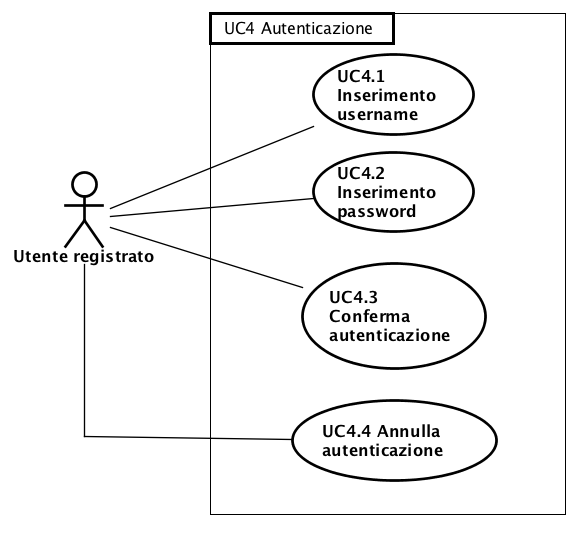
\includegraphics[scale=0.4]{diagram/UC4.png}
	\caption{Caso d'uso UC4}
	\end{center}
\end{figure}
\begin{itemize}
	\item \textbf{Precondizione:} il sistema ha selezionato la presentazione scelta dall'utente ed è in attesa di un'operazione da parte sua;
	\item \textbf{Postcondizione:} il sistema ha salvato le modifiche dell'utente;
	\item \textbf{Descrizione:} l'utente può modificare una presentazione scelta dall'elenco di quelle che ha creato;
	\item \textbf{Attori:} Utente autenticato;
	\item \textbf{Scenario principale:}
	\begin{enumerate}
		\item \textbf{ UC4.1:} \textit{ Inserimento oggetto grafico};
		\item \textbf{ UC4.2:} \textit{ Seleziona oggetto grafico};
		\item \textbf{ UC4.3:} \textit{ Modifica oggetto grafico};
		\item \textbf{ UC4.4:} \textit{ Elimina oggetto grafico};
		\item \textbf{ UC4.5:} \textit{ Crea percorso};
		\item \textbf{ UC4.6:} \textit{ Seleziona percorso};
		\item \textbf{ UC4.7:} \textit{ Modifica percorso};
		\item \textbf{ UC4.8:} \textit{ Elimina percorso};
		\item \textbf{ UC4.9:} \textit{ Modifica descrizione};
		\item \textbf{ UC4.10:} \textit{ Modifica titolo presentazione}.
	\end{enumerate}
\end{itemize}
\subsection{ UC4.1: Inserimento oggetto grafico}

\begin{figure}[h]
	\begin{center}
	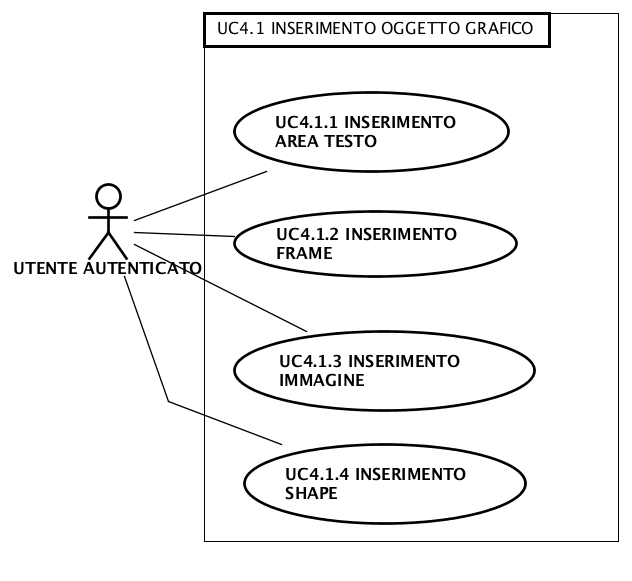
\includegraphics[scale=0.4]{diagram/UC4-1.png}
	\caption{Caso d'uso UC4.1}
	\end{center}
\end{figure}
\begin{itemize}
	\item \textbf{Precondizione:} il sistema è in fase di modifica della presentazione ed è in attesa di un'operazione da parte dell'utente;
	\item \textbf{Postcondizione:} il sistema ha aggiunto un oggetto grafico all'interno della presentazione, la modifica viene visualizzata;
	\item \textbf{Descrizione:} l'utente può aggiungere un oggetto grafico alla presentazione nella posizione predefinita;
	\item \textbf{Attori:} Utente autenticato;
	\item \textbf{Scenario principale:}
	\begin{enumerate}
		\item \textbf{ UC4.1.1:} \textit{ Inserimento area di testo};
		\item \textbf{ UC4.1.2:} \textit{ Inserimento frame};
		\item \textbf{ UC4.1.3:} \textit{ Inserimento immagine};
		\item \textbf{ UC4.1.4:} \textit{ Inserimento shape}.
	\end{enumerate}
\end{itemize}
\subsection{ UC4.1.1: Inserimento area di testo}

\begin{figure}[h]
	\begin{center}
	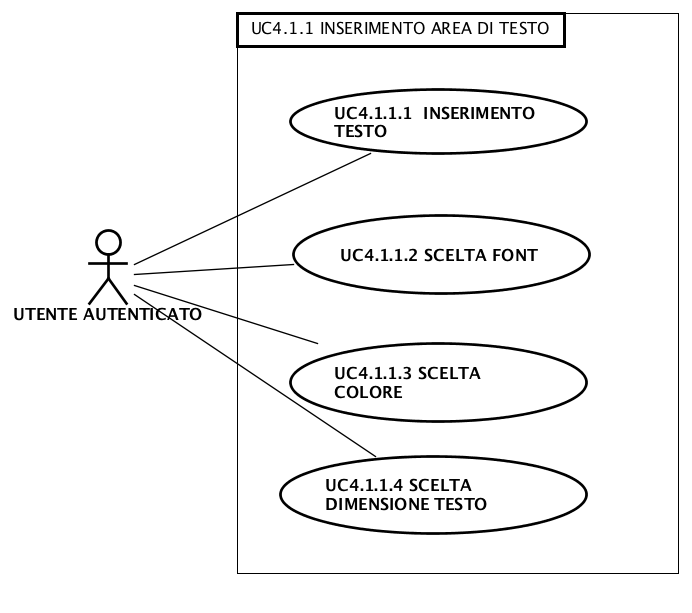
\includegraphics[scale=0.4]{diagram/UC4-1-1.png}
	\caption{Caso d'uso UC4.1.1}
	\end{center}
\end{figure}
\begin{itemize}
	\item \textbf{Precondizione:} il sistema è in fase di modifica della presentazione ed è in attesa di un'operazione da parte dell'utente;
	\item \textbf{Postcondizione:} il sistema ha aggiunto del testo all'interno della presentazione, la modifica viene visualizzata;
	\item \textbf{Descrizione:} l'utente può aggiungere un'area di testo all'interno della presentazione;
	\item \textbf{Attori:} Utente autenticato;
	\item \textbf{Scenario principale:}
	\begin{enumerate}
		\item \textbf{ UC4.1.1.1:} \textit{ Inserimento testo};
		\item \textbf{ UC4.1.1.2:} \textit{ Scelta font};
		\item \textbf{ UC4.1.1.3:} \textit{ Scelta colore};
		\item \textbf{ UC4.1.1.4:} \textit{ Scelta dimensione testo}.
	\end{enumerate}
\end{itemize}
\subsection{ UC4.1.1.1: Inserimento testo}

\begin{itemize}
	\item \textbf{Precondizione:} il sistema è in fase di modifica della presentazione ed è in attesa dell'inserimento del testo da parte dell'utente;
	\item \textbf{Postcondizione:} il sistema ha inserito il testo, viene visualizzata la modifica;
	\item \textbf{Descrizione:} l'utente può inserire del testo;
	\item \textbf{Attori:} Utente autenticato.
\end{itemize}
\subsection{ UC4.1.1.2: Scelta font}

\begin{itemize}
	\item \textbf{Precondizione:} il sistema è in fase di modifica della presentazione ed è in attesa della scelta di un font da parte dell'utente;
	\item \textbf{Postcondizione:} il sistema ha selezionato il font scelto dall'utente, viene visualizzata la modifica;
	\item \textbf{Descrizione:} l'utente può scegliere il font del testo;
	\item \textbf{Attori:} Utente autenticato.
\end{itemize}
\subsection{ UC4.1.1.3: Scelta colore}

\begin{itemize}
	\item \textbf{Precondizione:} il sistema è in fase di modifica della presentazione ed è in attesa della scelta di un colore da parte dell'utente;
	\item \textbf{Postcondizione:} il sistema ha applicato il colore scelto dall'utente, viene visualizzata la modifica;
	\item \textbf{Descrizione:} l'utente può scegliere il colore del testo;
	\item \textbf{Attori:} Utente autenticato.
\end{itemize}
\subsection{ UC4.1.1.4: Scelta dimensione testo}

\begin{itemize}
	\item \textbf{Precondizione:} il sistema è in fase di modifica della presentazione ed è in attesa della scelta della dimensione del testo da parte dell'utente;
	\item \textbf{Postcondizione:} il sistema ha applicato la dimensione scelta dall'utente, viene visualizzata la modifica;
	\item \textbf{Descrizione:} l'utente può scegliere la dimensione del testo;
	\item \textbf{Attori:} Utente autenticato.
\end{itemize}
\subsection{ UC4.1.2: Inserimento frame}

\begin{figure}[h]
	\begin{center}
	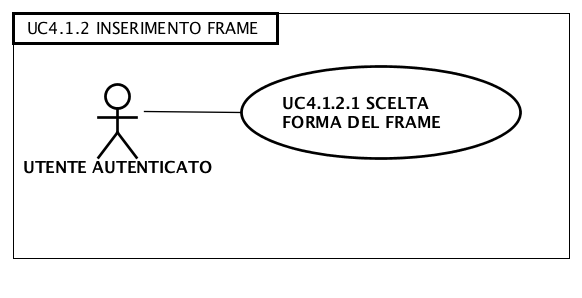
\includegraphics[scale=0.4]{diagram/UC4-1-2.png}
	\caption{Caso d'uso UC4.1.2}
	\end{center}
\end{figure}
\begin{itemize}
	\item \textbf{Precondizione:} il sistema è in fase di modifica della presentazione ed è in attesa di un'operazione da parte dell'utente;
	\item \textbf{Postcondizione:} il sistema ha aggiunto un frame all'interno della presentazione, la modifica viene visualizzata;
	\item \textbf{Descrizione:} l'utente può aggiungere un frame all'interno della presentazione;
	\item \textbf{Attori:} Utente autenticato;
	\item \textbf{Scenario principale:}
	\begin{enumerate}
		\item \textbf{ UC4.1.2.1:} \textit{ Scelta forma frame}.
	\end{enumerate}
\end{itemize}
\subsection{ UC4.1.2.1: Scelta forma frame}

\begin{itemize}
	\item \textbf{Precondizione:} il sistema è in fase di modifica della presentazione ed è in attesa della scelta di una forma da parte dell'utente;
	\item \textbf{Postcondizione:} il sistema ha selezionato la forma per il frame e viene visualizzata la modifica;
	\item \textbf{Descrizione:} l'utente può scegliere la forma del frame;
	\item \textbf{Attori:} Utente autenticato.
\end{itemize}
\subsection{ UC4.1.3: Inserimento immagine}

\begin{figure}[h]
	\begin{center}
	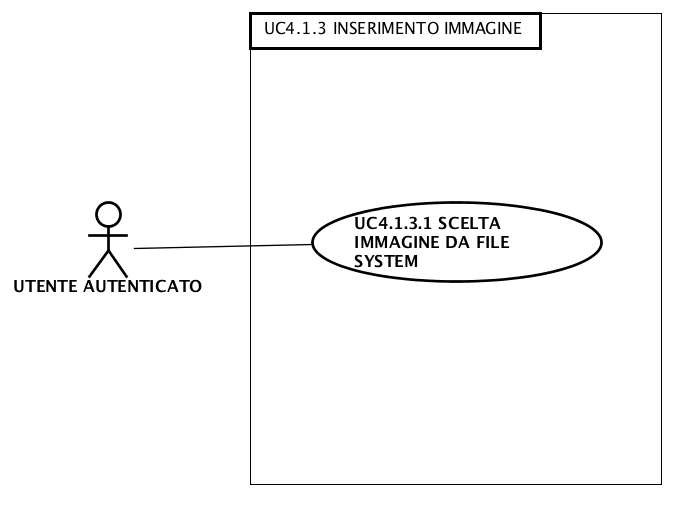
\includegraphics[scale=0.4]{diagram/UC4-1-3.png}
	\caption{Caso d'uso UC4.1.3}
	\end{center}
\end{figure}
\begin{itemize}
	\item \textbf{Precondizione:} il sistema è in fase di modifica della presentazione ed è in attesa di un'operazione da parte dell'utente;
	\item \textbf{Postcondizione:} il sistema ha aggiunto un'immagine all'interno della presentazione, la modifica viene visualizzata;
	\item \textbf{Descrizione:} l'utente può aggiungere un'immagine all'interno della presentazione;
	\item \textbf{Attori:} Utente autenticato;
	\item \textbf{Scenario principale:}
	\begin{enumerate}
		\item \textbf{ UC4.1.3.1:} \textit{ Scelta immagine da filesystem}.
	\end{enumerate}
\end{itemize}
\subsection{ UC4.1.3.1: Scelta immagine da filesystem}

\begin{itemize}
	\item \textbf{Precondizione:} il sistema è in fase di modifica della presentazione ed è in attesa della scelta dell'immagine da parte dell'utente;
	\item \textbf{Postcondizione:} il sistema ha selezionato l'immagine da filesystem, e ha visualizzato le modifiche;
	\item \textbf{Descrizione:} l'utente deve poter selezionare un immagine da filesystem;
	\item \textbf{Attori:} Utente autenticato.
\end{itemize}
\subsection{ UC4.1.4: Inserimento shape}

\begin{figure}[h]
	\begin{center}
	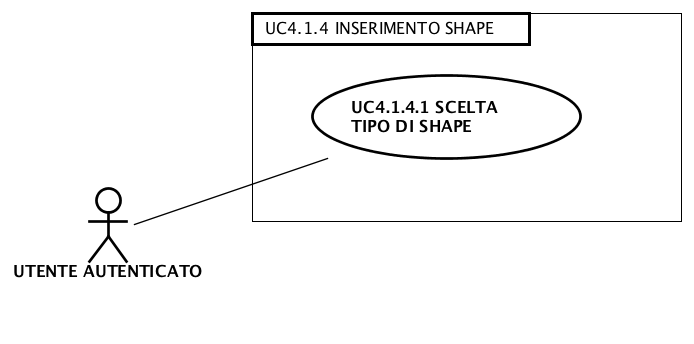
\includegraphics[scale=0.4]{diagram/UC4-1-4.png}
	\caption{Caso d'uso UC4.1.4}
	\end{center}
\end{figure}
\begin{itemize}
	\item \textbf{Precondizione:} il sistema è in fase di modifica della presentazione ed è in attesa di un'operazione da parte dell'utente;
	\item \textbf{Postcondizione:} il sistema ha aggiunto uno shape all'interno della presentazione, la modifica viene visualizzata;
	\item \textbf{Descrizione:} l'utente può aggiungere uno shape all'interno della presentazione;
	\item \textbf{Attori:} Utente autenticato;
	\item \textbf{Scenario principale:}
	\begin{enumerate}
		\item \textbf{ UC4.1.4.1:} \textit{ Scelta tipo shape}.
	\end{enumerate}
\end{itemize}
\subsection{ UC4.1.4.1: Scelta tipo shape}

\begin{itemize}
	\item \textbf{Precondizione:} il sistema è in fase di modifica della presentazione ed è in attesa della scelta di un tipo di shape da parte dell'utente;
	\item \textbf{Postcondizione:} il sistema ha selezionato la tipologia di shape, e viene visualizzata la modifica;
	\item \textbf{Descrizione:} l'utente può scegliere il tipo di shape;
	\item \textbf{Attori:} Utente autenticato.
\end{itemize}
\subsection{ UC4.2: Seleziona oggetto grafico}

\begin{itemize}
	\item \textbf{Precondizione:} il sistema è in fase di modifica della presentazione ed è in attesa di un'operazione da parte dell'utente;
	\item \textbf{Postcondizione:} il sistema ha selezionato un oggetto grafico;
	\item \textbf{Descrizione:} l'utente può selezionare un oggetto grafico;
	\item \textbf{Attori:} Utente autenticato.
\end{itemize}
\subsection{ UC4.3: Modifica oggetto grafico}

\begin{figure}[h]
	\begin{center}
	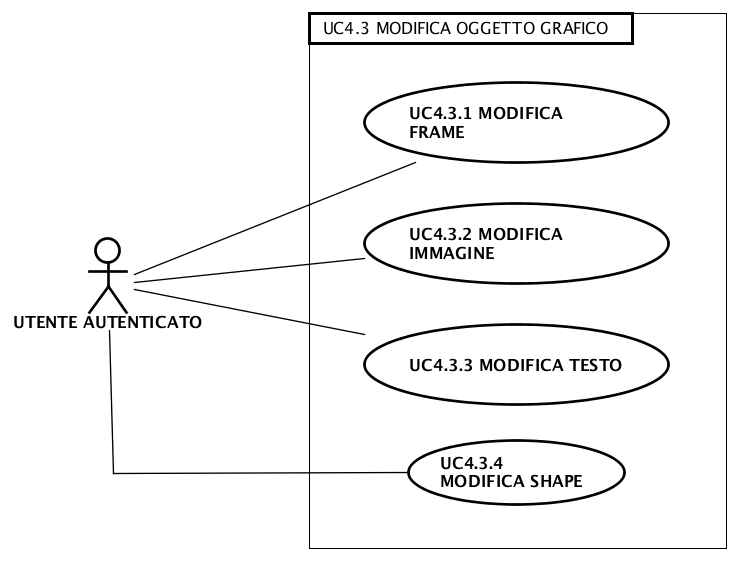
\includegraphics[scale=0.4]{diagram/UC4-3.png}
	\caption{Caso d'uso UC4.3}
	\end{center}
\end{figure}
\begin{itemize}
	\item \textbf{Precondizione:} il sistema è in fase di modifica della presentazione ed è in attesa di un'operazione da parte dell'utente;
	\item \textbf{Postcondizione:} il sistema ha modificato un oggetto grafico all'interno della presentazione, la modifica viene visualizzata;
	\item \textbf{Descrizione:} l'utente può modificare un oggetto grafico;
	\item \textbf{Attori:} Utente autenticato;
	\item \textbf{Scenario principale:}
	\begin{enumerate}
		\item \textbf{ UC4.3.1:} \textit{ Modifica frame};
		\item \textbf{ UC4.3.2:} \textit{ Modifica immagine};
		\item \textbf{ UC4.3.3:} \textit{ Modifica area di testo};
		\item \textbf{ UC4.3.4:} \textit{ Modifica shape}.
	\end{enumerate}
\end{itemize}
\subsection{ UC4.3.1: Modifica frame}

\begin{figure}[h]
	\begin{center}
	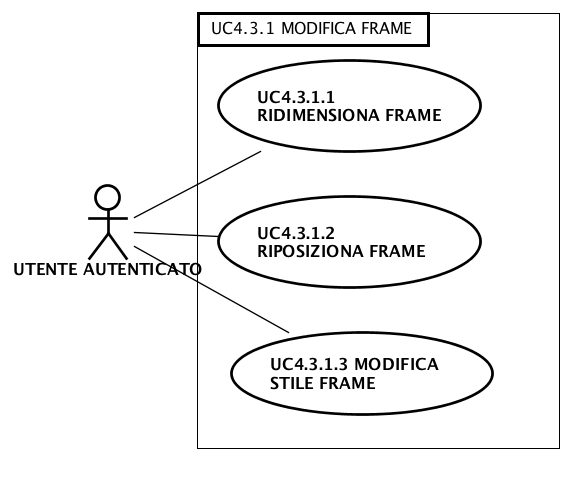
\includegraphics[scale=0.4]{diagram/UC4-3-1.png}
	\caption{Caso d'uso UC4.3.1}
	\end{center}
\end{figure}
\begin{itemize}
	\item \textbf{Precondizione:} il sistema è in fase di modifica della presentazione ed è stato selezionato un frame;
	\item \textbf{Postcondizione:} il sistema ha modificato il frame e viene visualizzata la modifica;
	\item \textbf{Descrizione:} l'utente può modificare un frame;
	\item \textbf{Attori:} Utente autenticato;
	\item \textbf{Scenario principale:}
	\begin{enumerate}
		\item \textbf{ UC4.3.1.1:} \textit{ Ridimensiona frame};
		\item \textbf{ UC4.3.1.2:} \textit{ Riposiziona frame};
		\item \textbf{ UC4.3.1.3:} \textit{ Modifica stile frame}.
	\end{enumerate}
\end{itemize}
\subsection{ UC4.3.1.1: Ridimensiona frame}

\begin{itemize}
	\item \textbf{Precondizione:} il sistema è in fase di modifica della presentazione ed è stato selezionato un frame;
	\item \textbf{Postcondizione:} il sistema ha ridimensionato il frame e viene visualizzata la modifica;
	\item \textbf{Descrizione:} l'utente può ridimensionare un frame;
	\item \textbf{Attori:} Utente autenticato.
\end{itemize}
\subsection{ UC4.3.1.2: Riposiziona frame}

\begin{itemize}
	\item \textbf{Precondizione:} il sistema è in fase di modifica della presentazione ed è stato selezionato un frame;
	\item \textbf{Postcondizione:} il sistema ha riposizionato il frame e viene visualizzata la modifica;
	\item \textbf{Descrizione:} l'utente può riposizionare un frame;
	\item \textbf{Attori:} Utente autenticato.
\end{itemize}
\subsection{ UC4.3.1.3: Modifica stile frame}

\begin{itemize}
	\item \textbf{Precondizione:} il sistema è in fase di modifica della presentazione ed è stato selezionato un frame;
	\item \textbf{Postcondizione:} il sistema ha modificato lo stile del frame e viene visualizzata la modifica;
	\item \textbf{Descrizione:} l'utente può modificare lo stile di un frame;
	\item \textbf{Attori:} Utente autenticato.
\end{itemize}
\subsection{ UC4.3.2: Modifica immagine}

\begin{figure}[h]
	\begin{center}
	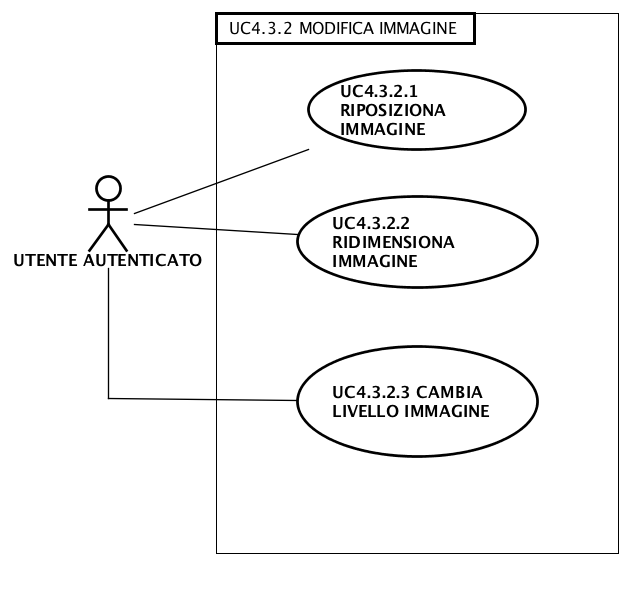
\includegraphics[scale=0.4]{diagram/UC4-3-2.png}
	\caption{Caso d'uso UC4.3.2}
	\end{center}
\end{figure}
\begin{itemize}
	\item \textbf{Precondizione:} il sistema è in fase di modifica della presentazione ed è stata selezionata un'immagine;
	\item \textbf{Postcondizione:} il sistema ha modificato l'immagine e viene visualizzata la modifica;
	\item \textbf{Descrizione:} l'utente può modificare un'immagine;
	\item \textbf{Attori:} Utente autenticato;
	\item \textbf{Scenario principale:}
	\begin{enumerate}
		\item \textbf{ UC4.3.2.1:} \textit{ Riposiziona immagine};
		\item \textbf{ UC4.3.2.2:} \textit{ Ridimensiona immagine};
		\item \textbf{ UC4.3.2.3:} \textit{ Cambia livello immagine}.
	\end{enumerate}
\end{itemize}
\subsection{ UC4.3.2.1: Riposiziona immagine}

\begin{itemize}
	\item \textbf{Precondizione:} il sistema è in fase di modifica della presentazione ed è stata selezionata un'immagine;
	\item \textbf{Postcondizione:} il sistema ha riposizionato l'immagine e viene visualizzata la modifica;
	\item \textbf{Descrizione:} l'utente può riposizionare un'immagine;
	\item \textbf{Attori:} Utente autenticato.
\end{itemize}
\subsection{ UC4.3.2.2: Ridimensiona immagine}

\begin{itemize}
	\item \textbf{Precondizione:} il sistema è in fase di modifica della presentazione ed è stata selezionata un'immagine;
	\item \textbf{Postcondizione:} il sistema ha ridimensionato l'immagine e viene visualizzata la modifica;
	\item \textbf{Descrizione:} l'utente può ridimensionare un'immagine;
	\item \textbf{Attori:} Utente autenticato.
\end{itemize}
\subsection{ UC4.3.2.3: Cambia livello immagine}

\begin{itemize}
	\item \textbf{Precondizione:} il sistema è in fase di modifica della presentazione ed è stata selezionata un'immagine;
	\item \textbf{Postcondizione:} il sistema ha cambiato il livello dell'immagine e viene visualizzata la modifica;
	\item \textbf{Descrizione:} l'utente può cambiare il livello dell'immagine selezionata;
	\item \textbf{Attori:} Utente autenticato.
\end{itemize}
\subsection{ UC4.3.3: Modifica area di testo}

\begin{figure}[h]
	\begin{center}
	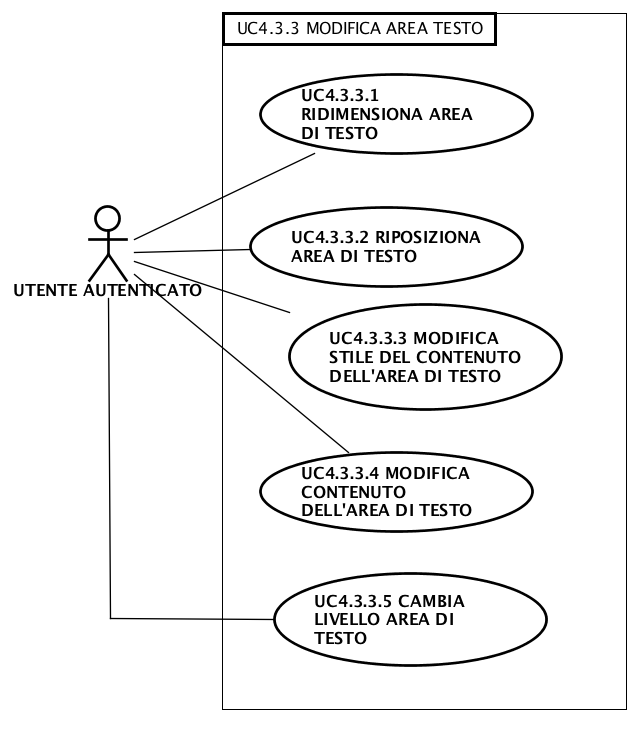
\includegraphics[scale=0.4]{diagram/UC4-3-3.png}
	\caption{Caso d'uso UC4.3.3}
	\end{center}
\end{figure}
\begin{itemize}
	\item \textbf{Precondizione:} il sistema è in fase di modifica della presentazione ed è stato selezionato un testo;
	\item \textbf{Postcondizione:} il sistema ha modificato il testo e viene visualizzata la modifica;
	\item \textbf{Descrizione:} l'utente può modificare un testo;
	\item \textbf{Attori:} Utente autenticato;
	\item \textbf{Scenario principale:}
	\begin{enumerate}
		\item \textbf{ UC4.3.3.1:} \textit{ Ridimensiona area di testo};
		\item \textbf{ UC4.3.3.2:} \textit{ Riposiziona area di testo};
		\item \textbf{ UC4.3.3.3:} \textit{ Modifica stile del contenuto dell'area di testo};
		\item \textbf{ UC4.3.3.4:} \textit{ Modifica contenuto dell'area di testo};
		\item \textbf{ UC4.3.3.5:} \textit{ Cambia livello area di testo}.
	\end{enumerate}
\end{itemize}
\subsection{ UC4.3.3.1: Ridimensiona area di testo}

\begin{itemize}
	\item \textbf{Precondizione:} il sistema è in fase di modifica della presentazione ed è stata selezionata un'area di testo;
	\item \textbf{Postcondizione:} il sistema ha ridimensionato l'area di testo e viene visualizzata la modifica;
	\item \textbf{Descrizione:} l'utente può ridimensionare un'area di testo;
	\item \textbf{Attori:} Utente autenticato.
\end{itemize}
\subsection{ UC4.3.3.2: Riposiziona area di testo}

\begin{itemize}
	\item \textbf{Precondizione:} il sistema è in fase di modifica della presentazione ed è stata selezionata un'area di testo;
	\item \textbf{Postcondizione:} il sistema ha riposizionato l'area di testo e viene visualizzata la modifica;
	\item \textbf{Descrizione:} l'utente può riposizionare un'area di testo;
	\item \textbf{Attori:} Utente autenticato.
\end{itemize}
\subsection{ UC4.3.3.3: Modifica stile del contenuto dell'area di testo}

\begin{itemize}
	\item \textbf{Precondizione:} il sistema è in fase di modifica della presentazione ed è stata selezionata un'area di testo;
	\item \textbf{Postcondizione:} il sistema ha modificato lo stile del contenuto dell'area di testo e viene visualizzata la modifica;
	\item \textbf{Descrizione:} l'utente può modificare lo stile del contenuto dell'area di testo;
	\item \textbf{Attori:} Utente autenticato.
\end{itemize}
\subsection{ UC4.3.3.4: Modifica contenuto dell'area di testo}

\begin{itemize}
	\item \textbf{Precondizione:} il sistema è in fase di modifica della presentazione ed è stata selezionata un'area di testo;
	\item \textbf{Postcondizione:} il sistema ha modificato il contenuto dell'area di testo e viene visualizzata la modifica;
	\item \textbf{Descrizione:} l'utente può modificare il contenuto dell'area di testo;
	\item \textbf{Attori:} Utente autenticato.
\end{itemize}
\subsection{ UC4.3.3.5: Cambia livello area di testo}

\begin{itemize}
	\item \textbf{Precondizione:} il sistema è in fase di modifica della presentazione ed è stata selezionata un'area di testo;
	\item \textbf{Postcondizione:} il sistema ha cambiato il livello dell'area di testo e viene visualizzata la modifica;
	\item \textbf{Descrizione:} l'utente può cambiare il livello dell'area di testo selezionata;
	\item \textbf{Attori:} Utente autenticato.
\end{itemize}
\subsection{ UC4.3.4: Modifica shape}

\begin{figure}[h]
	\begin{center}
	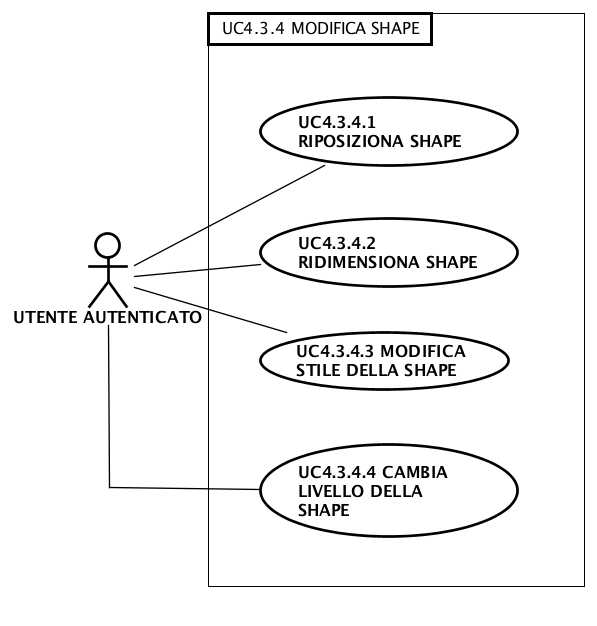
\includegraphics[scale=0.4]{diagram/UC4-3-4.png}
	\caption{Caso d'uso UC4.3.4}
	\end{center}
\end{figure}
\begin{itemize}
	\item \textbf{Precondizione:} il sistema è in fase di modifica della presentazione ed è stato selezionato una shape;
	\item \textbf{Postcondizione:} il sistema ha modificato la shape e viene visualizzata la modifica;
	\item \textbf{Descrizione:} l'utente può modificare una shape;
	\item \textbf{Attori:} Utente autenticato;
	\item \textbf{Scenario principale:}
	\begin{enumerate}
		\item \textbf{ UC4.3.4.1:} \textit{ Riposiziona shape};
		\item \textbf{ UC4.3.4.2:} \textit{ Ridimensiona shape};
		\item \textbf{ UC4.3.4.3:} \textit{ Modifica stile della shape};
		\item \textbf{ UC4.3.4.4:} \textit{ Cambia livello alla shape}.
	\end{enumerate}
\end{itemize}
\subsection{ UC4.3.4.1: Riposiziona shape}

\begin{itemize}
	\item \textbf{Precondizione:} 	il sistema è in fase di modifica della presentazione ed è stato selezionato una shape;
	\item \textbf{Postcondizione:} il sistema ha riposizionato la shape e viene visualizzata la modifica;
	\item \textbf{Descrizione:} l'utente puòriposizionare la shape selezionata;
	\item \textbf{Attori:} Utente autenticato.
\end{itemize}
\subsection{ UC4.3.4.2: Ridimensiona shape}

\begin{itemize}
	\item \textbf{Precondizione:} il sistema è in fase di modifica della presentazione ed è stata selezionata una shape;
	\item \textbf{Postcondizione:} il sistema ha ridimensionato la shape e viene visualizzata la modifica;
	\item \textbf{Descrizione:} l'utente può ridimensionare una shape;
	\item \textbf{Attori:} Utente autenticato.
\end{itemize}
\subsection{ UC4.3.4.3: Modifica stile della shape}

\begin{itemize}
	\item \textbf{Precondizione:} il sistema è in fase di modifica della presentazione ed è stata selezionata una shape;
	\item \textbf{Postcondizione:} il sistema ha modificato lo stile della shape e viene visualizzata la modifica;
	\item \textbf{Descrizione:} l'utente può modificare lo stile della shape selezionata;
	\item \textbf{Attori:} Utente autenticato.
\end{itemize}
\subsection{ UC4.3.4.4: Cambia livello alla shape}

\begin{itemize}
	\item \textbf{Precondizione:} ;
	\item \textbf{Postcondizione:} ;
	\item \textbf{Descrizione:} ;
	\item \textbf{Attori:} Utente autenticato.
\end{itemize}
\subsection{ UC4.4: Elimina oggetto grafico}

\begin{itemize}
	\item \textbf{Precondizione:} il sistema è in fase di modifica della presentazione ed è stato selezionato un oggetto grafico;
	\item \textbf{Postcondizione:} il sistema ha eliminato l'oggetto grafico e viene visualizzata la modifica;
	\item \textbf{Descrizione:} l'utente può eliminare un oggetto grafico;
	\item \textbf{Attori:} Utente autenticato.
\end{itemize}
\subsection{ UC4.5: Crea percorso}

\begin{figure}[h]
	\begin{center}
	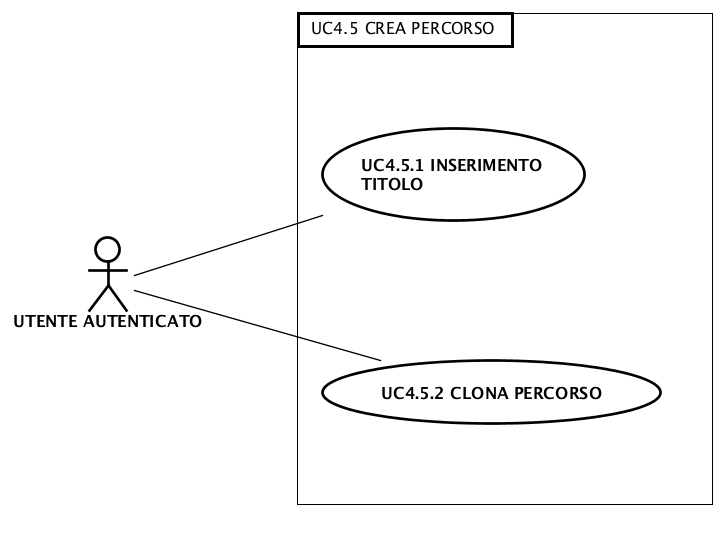
\includegraphics[scale=0.4]{diagram/UC4-5.png}
	\caption{Caso d'uso UC4.5}
	\end{center}
\end{figure}
\begin{itemize}
	\item \textbf{Precondizione:} il sistema è in fase di modifica della presentazione;
	\item \textbf{Postcondizione:} il sistema ha creato un nuovo percorso;
	\item \textbf{Descrizione:} l'utente può creare un nuovo percorso che descrive la successione dei frame durante l'esecuzione della presentazione;
	\item \textbf{Attori:} Utente autenticato;
	\item \textbf{Scenario principale:}
	\begin{enumerate}
		\item \textbf{ UC4.5.1:} \textit{ Inserimento titolo};
		\item \textbf{ UC4.5.2:} \textit{ Clona percorso}.
	\end{enumerate}
\end{itemize}
\subsection{ UC4.5.1: Inserimento titolo}

\begin{itemize}
	\item \textbf{Precondizione:} il sistema è in fase di modifica della presentazione ed è in attesa dell'inserimento di una descrizione;
	\item \textbf{Postcondizione:} il sistema ha inserito un titolo per il nuovo percorso;
	\item \textbf{Descrizione:} l'utente deve inserire un titolo per il nuovo percorso;
	\item \textbf{Attori:} Utente autenticato.
\end{itemize}
\subsection{ UC4.5.2: Clona percorso}

\begin{itemize}
	\item \textbf{Precondizione:} il sistema è in fase di modifica della presentazione ed è in attesa di un'operazione da parte dell'utente. Deve esistere almeno un percorso per la presentazione;
	\item \textbf{Postcondizione:} il sistema ha clonato un percorso scelto dall'utente;
	\item \textbf{Descrizione:} l'utente può clonare un percorso;
	\item \textbf{Attori:} Utente autenticato.
\end{itemize}
\subsection{ UC4.6: Seleziona percorso}

\begin{itemize}
	\item \textbf{Precondizione:} il sistema è in fase di modifica della presentazione ed è in attesa di un'operazione da parte dell'utente. Deve esistere almeno un percorso per la presentazione;
	\item \textbf{Postcondizione:} il sistema ha selezionato il percorso scelto dall'utente per la presentazione;
	\item \textbf{Descrizione:} l'utente può selezionare un percorso esistente nella presentazione;
	\item \textbf{Attori:} Utente autenticato.
\end{itemize}
\subsection{ UC4.7: Modifica percorso}

\begin{figure}[h]
	\begin{center}
	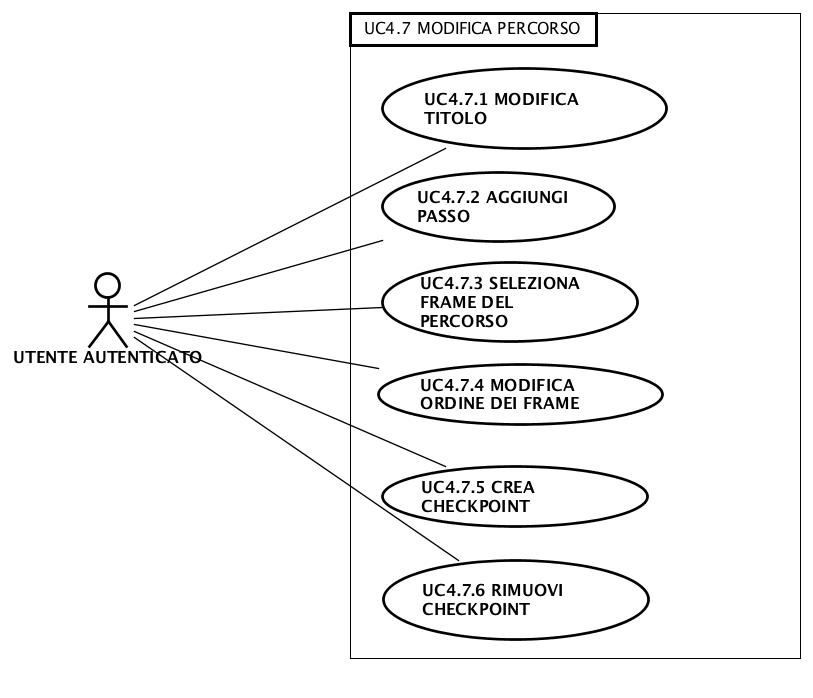
\includegraphics[scale=0.4]{diagram/UC4-7.png}
	\caption{Caso d'uso UC4.7}
	\end{center}
\end{figure}
\begin{itemize}
	\item \textbf{Precondizione:} il sistema è in fase di modifica della presentazione ed è stato selezionato un percorso;
	\item \textbf{Postcondizione:} il sistema ha modificato il percorso e viene visualizzata la modifica.;
	\item \textbf{Descrizione:} l'utente può modificare il percorso selezionato;
	\item \textbf{Attori:} Utente autenticato;
	\item \textbf{Scenario principale:}
	\begin{enumerate}
		\item \textbf{ UC4.7.1:} \textit{ Modifica titolo };
		\item \textbf{ UC4.7.2:} \textit{ Aggiungi passo};
		\item \textbf{ UC4.7.3:} \textit{ Seleziona frame del percorso};
		\item \textbf{ UC4.7.4:} \textit{ Modifica ordine dei frame};
		\item \textbf{ UC4.7.5:} \textit{ Crea checkpoint};
		\item \textbf{ UC4.7.6:} \textit{ Rimuovi checkpoint}.
	\end{enumerate}
\end{itemize}
\subsection{ UC4.7.1: Modifica titolo }

\begin{itemize}
	\item \textbf{Precondizione:} il sistema è in fase di modifica della presentazione ed è stato selezionato un percorso;
	\item \textbf{Postcondizione:} il sistema ha modificato il titolo per il percorso selezionato e viene visualizzata la modifica;
	\item \textbf{Descrizione:} l'utente può cambiare il titolo del percorso selezionato. La modifica verrà visualizzata;
	\item \textbf{Attori:} Utente autenticato.
\end{itemize}
\subsection{ UC4.7.2: Aggiungi passo}

\begin{itemize}
	\item \textbf{Precondizione:} il sistema è in fase di modifica della presentazione ed è stato selezionato un percorso;
	\item \textbf{Postcondizione:} il sistema ha aggiunto un passo del percorso e viene visualizzata la modifica;
	\item \textbf{Descrizione:} l'utente può aggiungere un passo al cammino. Ogni passo è associato ad un frame;
	\item \textbf{Attori:} Utente autenticato.
\end{itemize}
\subsection{ UC4.7.3: Seleziona frame del percorso}

\begin{itemize}
	\item \textbf{Precondizione:} il sistema è in fase di modifica della presentazione ed è stato selezionato un percorso;
	\item \textbf{Postcondizione:} il sistema ha selezionato un frame del percorso;
	\item \textbf{Descrizione:} l'utente può selezionare un frame del percorso;
	\item \textbf{Attori:} Utente autenticato.
\end{itemize}
\subsection{ UC4.7.4: Modifica ordine dei frame}

\begin{itemize}
	\item \textbf{Precondizione:} il sistema è in fase di modifica della presentazione, è stato selezionato un percorso ed un frame al suo interno;
	\item \textbf{Postcondizione:} il sistema ha modificato l'ordine dei frame e viene visualizzata la modifica;
	\item \textbf{Descrizione:} l'utente può modificare l'ordine dei frame all'interno del percorso;
	\item \textbf{Attori:} Utente autenticato.
\end{itemize}
\subsection{ UC4.7.5: Crea checkpoint}

\begin{itemize}
	\item \textbf{Precondizione:} il sistema è in fase di modifica della presentazione, è stato selezionato un percorso ed un frame al suo interno. Il frame selezionato non è un checkpoint;
	\item \textbf{Postcondizione:} il sistema ha reso il frame un checkpoint e viene visualizzata la modifica;
	\item \textbf{Descrizione:} l'utente può marcare un frame come checkpoint;
	\item \textbf{Attori:} Utente autenticato.
\end{itemize}
\subsection{ UC4.7.6: Rimuovi checkpoint}

\begin{figure}[h]
	\begin{center}
	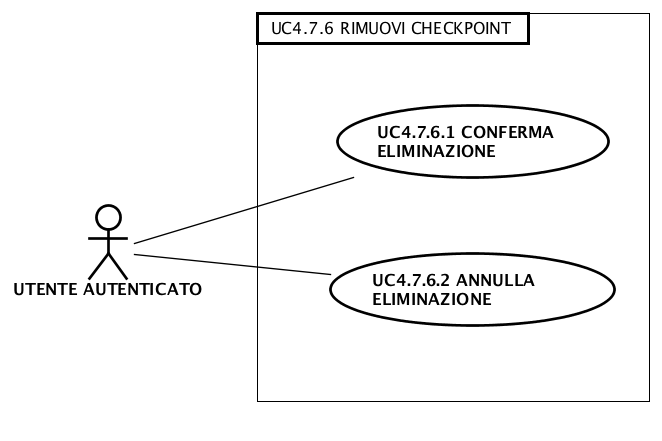
\includegraphics[scale=0.4]{diagram/UC4-7-6.png}
	\caption{Caso d'uso UC4.7.6}
	\end{center}
\end{figure}
\begin{itemize}
	\item \textbf{Precondizione:} il sistema è in fase di modifica della presentazione, è stato selezionato un percorso ed un frame al suo interno. Il frame selezionato è un checkpoint;
	\item \textbf{Postcondizione:} il sistema ha rimosso il checkpoint dal frame e viene visualizzata la modifica;
	\item \textbf{Descrizione:} l'utente può rimuovere checkpoint da un frame;
	\item \textbf{Attori:} Utente autenticato;
	\item \textbf{Scenario principale:}
	\begin{enumerate}
		\item \textbf{ UC4.7.6.1:} \textit{ Conferma eliminazione};
		\item \textbf{ UC4.7.6.2:} \textit{ Annulla eliminazione}.
	\end{enumerate}
\end{itemize}
\subsection{ UC4.7.6.1: Conferma eliminazione}

\begin{itemize}
	\item \textbf{Precondizione:} il sistema sta per eliminare un percorso, ed è in attesa di un'operazione da parte dell'utente;
	\item \textbf{Postcondizione:} il sistema ha ricevuto la conferma di eliminazione da parte dell'utente;
	\item \textbf{Descrizione:} l'utente può confermare l'eliminazione di un percorso;
	\item \textbf{Attori:} Utente autenticato.
\end{itemize}
\subsection{ UC4.7.6.2: Annulla eliminazione}

\begin{itemize}
	\item \textbf{Precondizione:} il sistema sta per eliminare un percorso, ed è in attesa di un'operazione da parte dell'utente;
	\item \textbf{Postcondizione:} il sistema ha ricevuto l'annullamento dell'eliminazione da parte dell'utente;
	\item \textbf{Descrizione:} l'utente può annullare l'eliminazione di un percorso;
	\item \textbf{Attori:} Utente autenticato.
\end{itemize}
\subsection{ UC4.8: Elimina percorso}

\begin{figure}[h]
	\begin{center}
	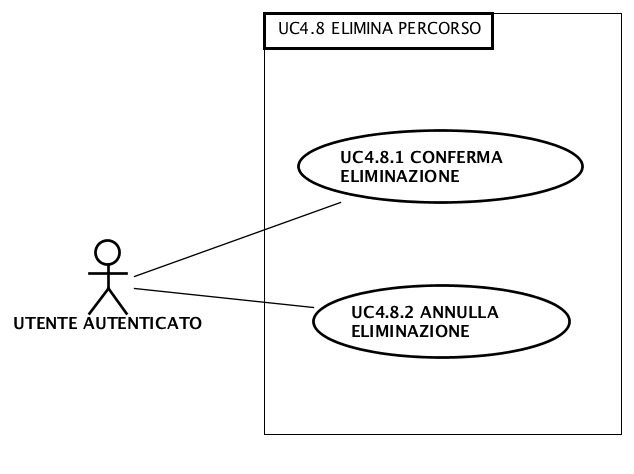
\includegraphics[scale=0.4]{diagram/UC4-8.png}
	\caption{Caso d'uso UC4.8}
	\end{center}
\end{figure}
\begin{itemize}
	\item \textbf{Precondizione:} ;
	\item \textbf{Postcondizione:} ;
	\item \textbf{Descrizione:} ;
	\item \textbf{Attori:} Utente autenticato;
	\item \textbf{Scenario principale:}
	\begin{enumerate}
		\item \textbf{ UC4.8.1:} \textit{ Conferma eliminazione};
		\item \textbf{ UC4.8.2:} \textit{ Annulla eliminazione}.
	\end{enumerate}
\end{itemize}
\subsection{ UC4.8.1: Conferma eliminazione}

\begin{itemize}
	\item \textbf{Precondizione:} ;
	\item \textbf{Postcondizione:} ;
	\item \textbf{Descrizione:} ;
	\item \textbf{Attori:} Utente autenticato.
\end{itemize}
\subsection{ UC4.8.2: Annulla eliminazione}

\begin{itemize}
	\item \textbf{Precondizione:} ;
	\item \textbf{Postcondizione:} ;
	\item \textbf{Descrizione:} ;
	\item \textbf{Attori:} Utente autenticato.
\end{itemize}
\subsection{ UC4.9: Modifica descrizione}

\begin{itemize}
	\item \textbf{Precondizione:} ;
	\item \textbf{Postcondizione:} ;
	\item \textbf{Descrizione:} ;
	\item \textbf{Attori:} Utente autenticato.
\end{itemize}
\subsection{ UC4.10: Modifica titolo presentazione}

\begin{itemize}
	\item \textbf{Precondizione:} ;
	\item \textbf{Postcondizione:} ;
	\item \textbf{Descrizione:} ;
	\item \textbf{Attori:} Utente autenticato.
\end{itemize}
\subsection{ UC5: Salva presentazione}

\begin{itemize}
	\item \textbf{Precondizione:} il sistema è in fase di modifica della presentazione, il sistema è in attesa di un'operazione da parte dell'utente;
	\item \textbf{Postcondizione:} il sistema ha salvato le modifiche della presentazione e viene visualizzato il salvataggio;
	\item \textbf{Descrizione:} l'utente dopo aver modificato una presentazione la può salvare;
	\item \textbf{Attori:} Utente autenticato.
\end{itemize}
\subsection{ UC6: Elimina presentazione}

\begin{figure}[h]
	\begin{center}
	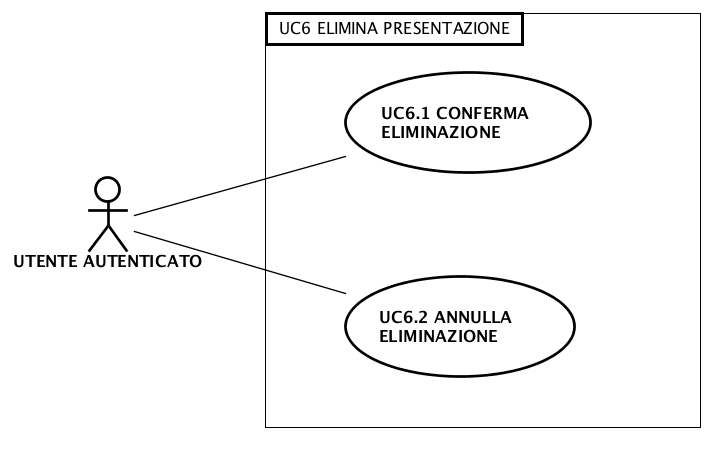
\includegraphics[scale=0.4]{diagram/UC6.png}
	\caption{Caso d'uso UC6}
	\end{center}
\end{figure}
\begin{itemize}
	\item \textbf{Precondizione:} il sistema ha selezionato la presentazione scelta dall'utente, ed è in attesa di un'operazione da parte dell'utente;
	\item \textbf{Postcondizione:} il sistema ha eliminato la presentazione e viene visualizzata la modifica;
	\item \textbf{Descrizione:} l'utente dopo aver selezionato una presentazione può eliminarla;
	\item \textbf{Attori:} Utente autenticato;
	\item \textbf{Scenario principale:}
	\begin{enumerate}
		\item \textbf{ UC6.1:} \textit{ Conferma eliminazione};
		\item \textbf{ UC6.2:} \textit{ Annulla eliminazione}.
	\end{enumerate}
\end{itemize}
\subsection{ UC6.1: Conferma eliminazione}

\begin{itemize}
	\item \textbf{Precondizione:} il sistema sta per eliminare una presentazione, ed è in attesa di un'operazione da parte dell'utente;
	\item \textbf{Postcondizione:} il sistema ha ricevuto la conferma di eliminazione da parte dell'utente;
	\item \textbf{Descrizione:} l'utente può confermare l'eliminazione di una presentazione;
	\item \textbf{Attori:} Utente autenticato.
\end{itemize}
\subsection{ UC6.2: Annulla eliminazione}

\begin{itemize}
	\item \textbf{Precondizione:} il sistema sta per eliminare una presentazione, ed è in attesa di un'operazione da parte dell'utente;
	\item \textbf{Postcondizione:} il sistema ha ricevuto l'annullamento dell'eliminazione da parte dell'utente;
	\item \textbf{Descrizione:} l'utente può annullare l'eliminazione di una presentazione;
	\item \textbf{Attori:} Utente autenticato.
\end{itemize}
\subsection{ UC7: Pubblica presentazione}

\begin{itemize}
	\item \textbf{Precondizione:} il sistema ha selezionato la presentazione scelta dall'utente. La presentazione selezionata è privata. Il sistema è in attesa di un'operazione da parte dell'utente;
	\item \textbf{Postcondizione:} il sistema ha pubblicato la presentazione, viene generato un link per la presentazione;
	\item \textbf{Descrizione:} l'utente può rendere pubblica una presentazione;
	\item \textbf{Attori:} Utente autenticato.
\end{itemize}
\subsection{ UC8: Visualizza link della presentazione pubblica}

\begin{itemize}
	\item \textbf{Precondizione:} il sistema ha selezionato la presentazione scelta dall'utente, e la presentazione è stata pubblicata;
	\item \textbf{Postcondizione:} il sistema visualizza il link;
	\item \textbf{Descrizione:} l'utente può visualizzare un link per la presentazione pubblica;
	\item \textbf{Attori:} Utente autenticato.
\end{itemize}
\subsection{ UC9: Rendi privata la presentazione}

\begin{itemize}
	\item \textbf{Precondizione:} il sistema ha selezionato la presentazione scelta dall'utente. La presentazione selezionata è pubblica. Il sistema è in attesa di un'operazione da parte dell'utente;
	\item \textbf{Postcondizione:} il sistema ha reso privata la presentazione;
	\item \textbf{Descrizione:} l'utente può rendere privata una presentazione pubblica;
	\item \textbf{Attori:} Utente autenticato.
\end{itemize}
\subsection{ UC10: Rendi live la presentazione}

\begin{itemize}
	\item \textbf{Precondizione:} il sistema ha selezionato la presentazione scelta dall'utente. La presentazione selezionata è pubblica. Il sistema è in attesa di un'operazione da parte dell'utente;
	\item \textbf{Postcondizione:} il sistema ha reso live la presentazione;
	\item \textbf{Descrizione:} l'utente può rendere live la presentazione;
	\item \textbf{Attori:} Utente autenticato.
\end{itemize}
\subsection{ UC11: Esporta presentazione}

\begin{figure}[h]
	\begin{center}
	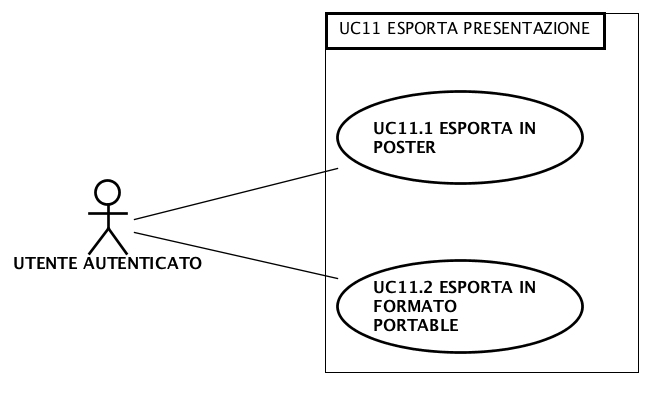
\includegraphics[scale=0.4]{diagram/UC11.png}
	\caption{Caso d'uso UC11}
	\end{center}
\end{figure}
\begin{itemize}
	\item \textbf{Precondizione:} il sistema ha selezionato la presentazione scelta dall'utente, ed è in attesa di un'operazione da parte dell'utente;
	\item \textbf{Postcondizione:} il sistema ha esportato la presentazione;
	\item \textbf{Descrizione:} l'utente può esportare la presentazione scelta;
	\item \textbf{Attori:} Utente autenticato;
	\item \textbf{Scenario principale:}
	\begin{enumerate}
		\item \textbf{ UC11.1:} \textit{ Esporta in poster};
		\item \textbf{ UC11.2:} \textit{ Esporta in formato portabile}.
	\end{enumerate}
\end{itemize}
\subsection{ UC11.1: Esporta in poster}

\begin{itemize}
	\item \textbf{Precondizione:} il sistema ha preso in carico l'esportazione della presentazione scelta dall'utente, ed è in attesa di un'operazione da parte dell'utente;
	\item \textbf{Postcondizione:} il sistema ha esportato la presentazione in poster e viene effettuato il download;
	\item \textbf{Descrizione:} l'utente può scegliere di esportare in poster la presentazione scelta;
	\item \textbf{Attori:} Utente autenticato.
\end{itemize}
\subsection{ UC11.2: Esporta in formato portabile}

\begin{itemize}
	\item \textbf{Precondizione:} il sistema ha preso in carico l'esportazione della presentazione scelta dall'utente, ed è in attesa di un'operazione da parte dell'utente;
	\item \textbf{Postcondizione:} il sistema ha esportato la presentazione in formato portable e viene effettuato il download;
	\item \textbf{Descrizione:} l'utente può scegliere di esportare in formato portable la presentazione scelta;
	\item \textbf{Attori:} Utente autenticato.
\end{itemize}
\subsection{ UC12: Partecipa a presentazione live}

\begin{itemize}
	\item \textbf{Precondizione:} il sistema si è collegato alla presentazione scelta dall'utente tramite un link di una presentazione pubblica;
	\item \textbf{Postcondizione:} il sistema ha visualizzato la presentazione;
	\item \textbf{Descrizione:} l'utente può collegarsi e visualizzare una presentazione pubblica;
	\item \textbf{Attori:} Utente autenticato.
\end{itemize}
\subsection{ UC13: Registrazione}

\begin{figure}[h]
	\begin{center}
	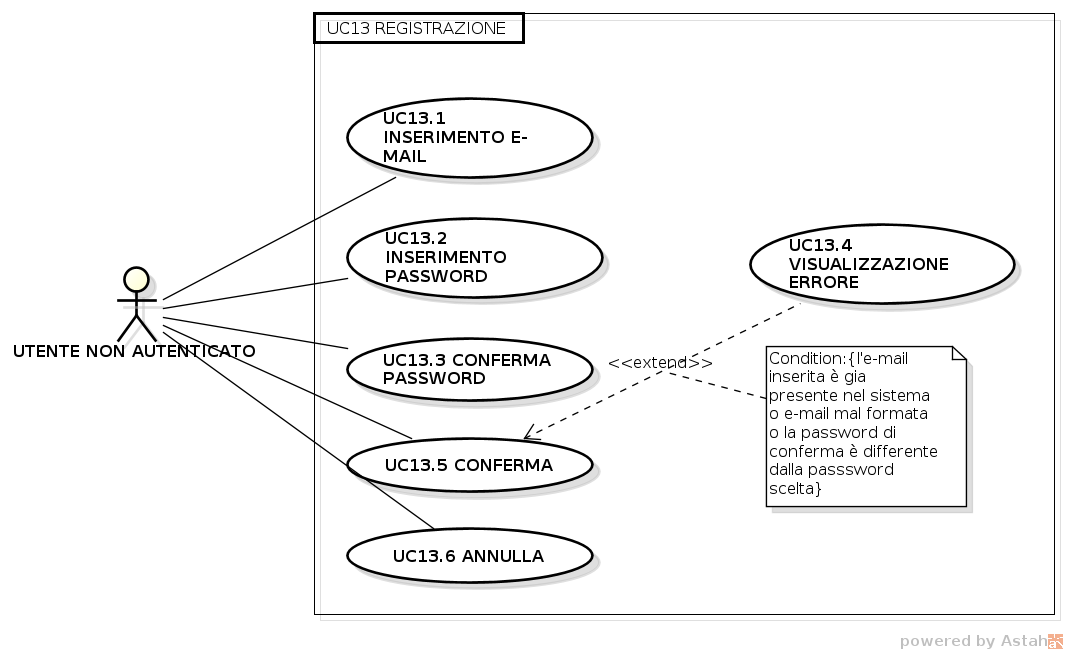
\includegraphics[scale=0.4]{diagram/UC13.png}
	\caption{Caso d'uso UC13}
	\end{center}
\end{figure}
\begin{itemize}
	\item \textbf{Precondizione:} il sistema è in attesa di un'operazione da parte dell'utente;
	\item \textbf{Postcondizione:} il sistema ha effettuato la registrazione dell'utente;
	\item \textbf{Descrizione:} l'utente può registrarsi al sistema;
	\item \textbf{Attori:} Utente non autenticato;
	\item \textbf{Scenario principale:}
	\begin{enumerate}
		\item \textbf{ UC13.1:} \textit{ Inserimento email};
		\item \textbf{ UC13.2:} \textit{ Inserimento password};
		\item \textbf{ UC13.3:} \textit{ Conferma password};
		\item \textbf{ UC13.4:} \textit{ Visualizza errore}.
	\end{enumerate}
\end{itemize}
\subsection{ UC13.1: Inserimento email}

\begin{itemize}
	\item \textbf{Precondizione:} il sistema è in fase di registrazione dell'utente, ed è in attesa di un'operazione da parte dell'utente;
	\item \textbf{Postcondizione:} il sistema ha inserito l'indirizzo email dell'utente e ha visualizzato le modifiche;
	\item \textbf{Descrizione:} l'utente deve inserire un indirizzo email;
	\item \textbf{Attori:} Utente non autenticato.
\end{itemize}
\subsection{ UC13.2: Inserimento password}

\begin{itemize}
	\item \textbf{Precondizione:} il sistema è in fase di registrazione dell'utente, ed è in attesa di un'operazione da parte dell'utente;
	\item \textbf{Postcondizione:} il sistema ha inserito la password dell'utente e ha visualizzato le modifiche;
	\item \textbf{Descrizione:} l'utente deve inserire una password;
	\item \textbf{Attori:} Utente non autenticato.
\end{itemize}
\subsection{ UC13.3: Conferma password}

\begin{itemize}
	\item \textbf{Precondizione:} il sistema è in fase di registrazione dell'utente, ed è in attesa di un'operazione da parte dell'utente;
	\item \textbf{Postcondizione:} il sistema ha inserito la password di conferma dell'utente e ha visualizzato le modifiche;
	\item \textbf{Descrizione:} l'utente deve inserire una password di conferma;
	\item \textbf{Attori:} Utente non autenticato.
\end{itemize}
\subsection{ UC13.4: Visualizza errore}

\begin{itemize}
	\item \textbf{Precondizione:} il sistema è in fase di registrazione dell'utente, ed è stato commesso un errore da parte dell'utente nell'inserimento del campo richiesto;
	\item \textbf{Postcondizione:} il sistema ha visualizzato un errore di inserimento;
	\item \textbf{Descrizione:} il sistema visualizza un errore di inserimento per il campo compilato dall'utente;
	\item \textbf{Attori:} Utente non autenticato.
\end{itemize}
\subsection{ UC14: Autenticazione}

\begin{figure}[h]
	\begin{center}
	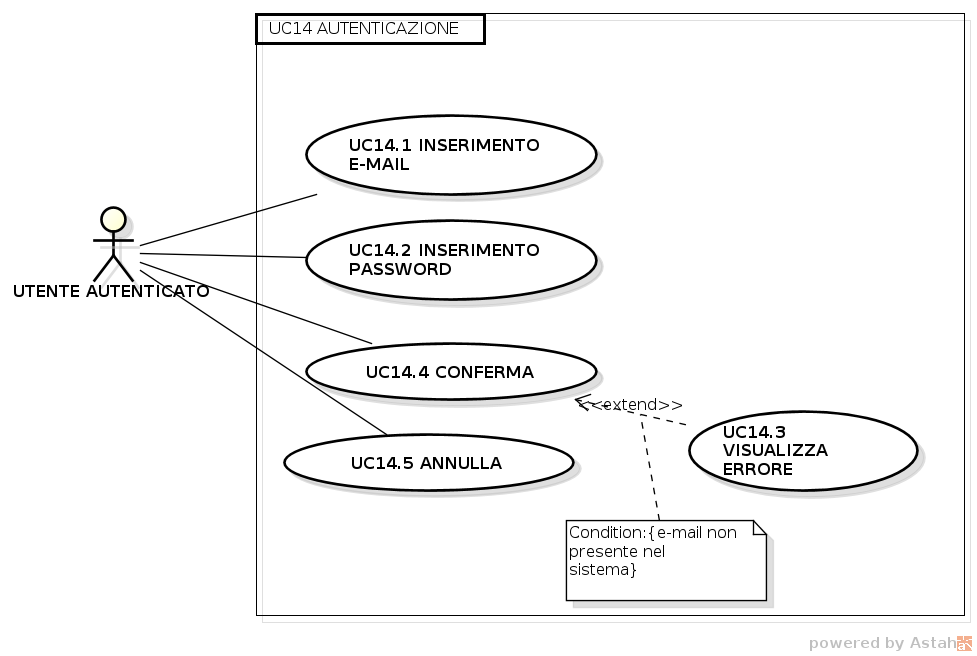
\includegraphics[scale=0.4]{diagram/UC14.png}
	\caption{Caso d'uso UC14}
	\end{center}
\end{figure}
\begin{itemize}
	\item \textbf{Precondizione:} il sistema è in attesa di un'operazione da parte dell'utente;
	\item \textbf{Postcondizione:} il sistema ha autenticato l'utente;
	\item \textbf{Descrizione:} l'utente può autenticarsi al sistema;
	\item \textbf{Attori:} Utente non autenticato;
	\item \textbf{Scenario principale:}
	\begin{enumerate}
		\item \textbf{ UC14.1:} \textit{ Inserimento email};
		\item \textbf{ UC14.2:} \textit{ Inserimento password};
		\item \textbf{ UC14.3:} \textit{ Visualizza errore}.
	\end{enumerate}
\end{itemize}
\subsection{ UC14.1: Inserimento email}

\begin{itemize}
	\item \textbf{Precondizione:} il sistema è in fase di autenticazione, ed è in attesa di un'operazione da parte dell'utente;
	\item \textbf{Postcondizione:} il sistema ha inserito l'indirizzo email dell'utente;
	\item \textbf{Descrizione:} l'utente deve inserire il proprio indirizzo email;
	\item \textbf{Attori:} Utente non autenticato.
\end{itemize}
\subsection{ UC14.2: Inserimento password}

\begin{itemize}
	\item \textbf{Precondizione:} il sistema è in fase di autenticazione, ed è in attesa di un'operazione da parte dell'utente;
	\item \textbf{Postcondizione:} il sistema ha inserito la password dell'utente;
	\item \textbf{Descrizione:} l'utente deve inserire una password;
	\item \textbf{Attori:} Utente non autenticato.
\end{itemize}
\subsection{ UC14.3: Visualizza errore}

\begin{itemize}
	\item \textbf{Precondizione:} il sistema è in fase di autenticazione dell'utente, ed è stato commesso un errore da parte dell'utente nell'inserimento del campo richiesto;
	\item \textbf{Postcondizione:} il sistema ha visualizzato un errore di inserimento;
	\item \textbf{Descrizione:} il sistema visualizza un errore di inserimento per il campo compilato dall'utente;
	\item \textbf{Attori:} Utente non autenticato.
\end{itemize}
\subsection{ UC15: Modifica password}

\begin{figure}[h]
	\begin{center}
	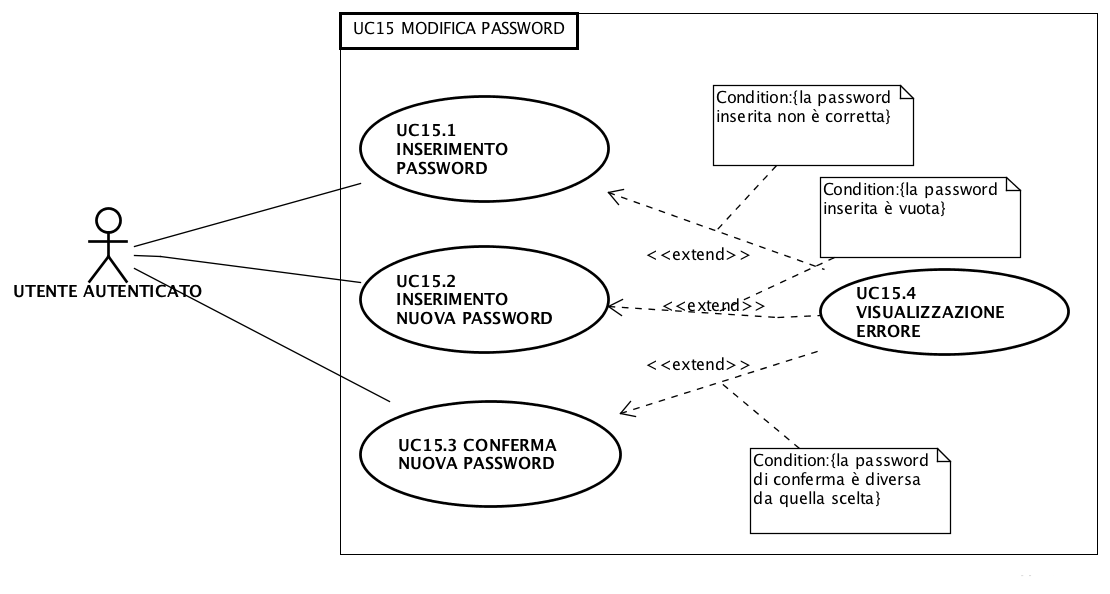
\includegraphics[scale=0.4]{diagram/UC15.png}
	\caption{Caso d'uso UC15}
	\end{center}
\end{figure}
\begin{itemize}
	\item \textbf{Precondizione:} il sistema è in attesa di un'operazione da parte dell'utente;
	\item \textbf{Postcondizione:} il sistema ha modificato la password dell'utente;
	\item \textbf{Descrizione:} l'utente può modificare la password;
	\item \textbf{Attori:} Utente autenticato;
	\item \textbf{Scenario principale:}
	\begin{enumerate}
		\item \textbf{ UC15.1:} \textit{ Inserimento password};
		\item \textbf{ UC15.2:} \textit{ Inserimento nuova password};
		\item \textbf{ UC15.3:} \textit{ Conferma nuova password};
		\item \textbf{ UC15.4:} \textit{ Visualizza errore}.
	\end{enumerate}
\end{itemize}
\subsection{ UC15.1: Inserimento password}

\begin{itemize}
	\item \textbf{Precondizione:} il sistema è in fase di modifica password, ed è in attesa di un'operazione da parte dell'utente;
	\item \textbf{Postcondizione:} il sistema ha inserito la password;
	\item \textbf{Descrizione:} l'utente deve inserire una password;
	\item \textbf{Attori:} Utente autenticato.
\end{itemize}
\subsection{ UC15.2: Inserimento nuova password}

\begin{itemize}
	\item \textbf{Precondizione:} il sistema è in fase di modifica password, ed è in attesa di un'operazione da parte dell'utente;
	\item \textbf{Postcondizione:} il sistema ha inserito una nuova password;
	\item \textbf{Descrizione:} l'utente deve inserire una nuova password;
	\item \textbf{Attori:} Utente autenticato.
\end{itemize}
\subsection{ UC15.3: Conferma nuova password}

\begin{itemize}
	\item \textbf{Precondizione:} il sistema è in fase di modifica password, ed è in attesa di un'operazione da parte dell'utente;
	\item \textbf{Postcondizione:} il sistema ha confermato la nuova password;
	\item \textbf{Descrizione:} l'utente deve inserire la conferma della nuova password;
	\item \textbf{Attori:} Utente autenticato.
\end{itemize}
\subsection{ UC15.4: Visualizza errore}

\begin{itemize}
	\item \textbf{Precondizione:} il sistema è in fase di di modifica password, ed è stato commesso un errore da parte dell'utente nell'inserimento del campo richiesto;
	\item \textbf{Postcondizione:} il sistema ha visualizzato un errore di inserimento;
	\item \textbf{Descrizione:} il sistema visualizza un errore di inserimento per il campo compilato dall'utente;
	\item \textbf{Attori:} Utente autenticato.
\end{itemize}